\section{Auswertung}
\label{sec:Auswertung}
\subsection{Berechnung der Brechungsindices $n_i$}
\subsubsection{Berechnung des \texorpdfstring{$\upvarphi$}{phi}-Winkels des verwendeten Prismas}

Für die Berechnung der Brechungsindices ist es notwendig zunächst den Winkel $\upvarphi$ zu bestimmen.
Seine Lage kann der Abbildung \ref{fig:Phi} entnommen werden.
Die Messwerte sind in Tabelle \ref{tab:Phi} zu finden.

\begin{table}
  \centering
  \caption{Gemessene Werte für $\upvarphi_{\text{r}}$ und $\upvarphi_{\text{l}}$, sowie die berechneten $\upvarphi$-Werte}
  \label{tab:Phi}
  \sisetup{table-format=3.1}
  \begin{tabular}{S S [table-format=3.1] S [table-format=2.2]}
    \toprule
    {$\upvarphi_{\text{r}} \:/\: \si{\degree}$} & {$\upvarphi_{\text{l}} \:/\: \si{\degree}$} & {$\upvarphi \:/\: \si{\degree}$} \\
    \midrule
    79.0  & 199.0 & 60.0  \\
    209.3 & 329.5 & 60.1  \\
    198.4 & 318.5 & 60.05 \\
    201.4 & 321.4 & 60.0  \\
    180.1 & 300.2 & 60.05 \\
    223.2 & 343.3 & 60.05 \\
    216.3 & 336.3 & 60.0  \\
    \bottomrule
  \end{tabular}
\end{table}

Um nun den eigentlichen Winkel $\upvarphi$ aus $\upvarphi_{\text{r}}$ und $\upvarphi_{\text{l}}$ der Tabelle \ref{tab:Phi} zu berechnen wird folgende Formel verwendet:

\begin{equation}
  \upvarphi = \frac{1}{2} \left(\upvarphi_r - \upvarphi_l\right)
\end{equation}

Der Mittelwert der errechneten $\upvarphi$ wird mit folgender Formel berechnet:

\begin{equation}
  \label{eqn:mittelwert}
  \overline{x} = \frac{1}{N} \sum_{i=1}^N x_i
\end{equation}

Der entsprechende Fehler mittels dieser:

\begin{equation}
  \label{eqn:mittelwertfehler}
  \Delta \overline{x} = \frac{1}{\sqrt{N}} \sqrt{\frac{1}{N-1} \sum_{i=1}^N (x_i - \overline{x})^2}
\end{equation}

Die Berechnungen erfolgen mit numpy und uncertainties.
Für $\upvarphi$ ergibt sich dann folgender Wert:

\begin{align*}
  \upvarphi &= \SI{60.04 \pm 0.01}{\degree}
\end{align*}

\subsubsection{Berechnung des \texorpdfstring{$\eta$}{eta}-Winkels des parallelen Strahlenganges}

\begin{figure}
  \centering
  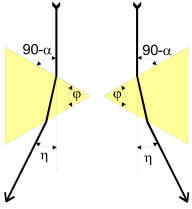
\includegraphics[scale=0.6]{images/Eta2.png}
  \caption{Der Brechungswinkel $\eta$: Aus der Anleitung des Versuches \cite[25]{1}}
  \label{fig:Eta2}
\end{figure}

Der Änderungswinkel $\eta$ des einfallenden Lichtstrahles ist in Abbildung \ref{fig:Eta2} dargestellt.
Auch dieser Winkel ist für die Bestimmung des Brechungsindex entscheidend.
Die Größen $\Omega_{\text{r}}$ und $\Omega_{\text{l}}$ der Tabelle \ref{tab:Eta} in denen die Messwerte aufgetragen sind, können der Abbildung \ref{fig:Drehung} entnommen werden.
Die entsprechenden Wellenlängen der Spektrallinien wurden der Quelle \cite{2} entnommen.
Das zugehörige im Experiment beobachtete Spektrum ist in Abbildung \ref{fig:spektrum} zu sehen.
Durch Vergleich der Wellenlängen aus \cite{2} mit denen aus Abbildung \ref{fig:Etatabelle} lassen sich
die gelbe, hellgrüne, hellviolette und violette Linie dem Quecksilber zuordnen.
Die rote, grüne, hellblaue  und blaue Linie stammen somit vom Cadmium.
Der Winkel $\eta$ berechnet sich dann nach der folgenden Formel:

\begin{equation}
  \eta = 180 - \left(\Omega_r - \Omega_l\right)
\end{equation}

Die Ergebnisse für die entsprechenden Wellenlängen $\lambda_i$ sind ebenfalls in Tabelle \ref{tab:Eta} enthalten.

\begin{table}
  \centering
  \caption{Gemessene Werte für $\Omega_{\text{r}}$ und $\Omega_{\text{l}}$}
  \label{tab:Eta}
  \sisetup{table-format=3.1}
  \begin{tabular}{S S S S [table-format=3.1] S [table-format=2.1]}
    \toprule
    {$\text{Farbe}$} & {$\lambda_i \:/\: \si{\nano\metre}$} & {$\Omega_{\text{r}} \:/\: \si{\degree}$} & {$\Omega_{\text{l}} \:/\: \si{\degree}$} & {$\eta_i \:/\: \si{\degree}$} \\
    \midrule
    \text{rot}         & 643.85 & 237.1 & 119.8 & 62.7 \\
    \text{gelb}        & 576.96 & 236.7 & 120.2 & 63.5 \\
    \text{hellgrün}    & 546.07 & 236.4 & 120.6 & 64.2 \\
    \text{grün}        & 508.58 & 235.8 & 121.1 & 65.3 \\
    \text{hellblau}    & 479.99 & 235.3 & 121.6 & 66.3 \\
    \text{blau}        & 467.82 & 235.1 & 121.9 & 66.8 \\
    \text{hellviolett} & 435.83 & 234.3 & 122.7 & 68.4 \\
    \text{violett}     & 404.65 & 233.3 & 123.7 & 70.4 \\
    \bottomrule
  \end{tabular}
\end{table}

\begin{figure}
  \centering
  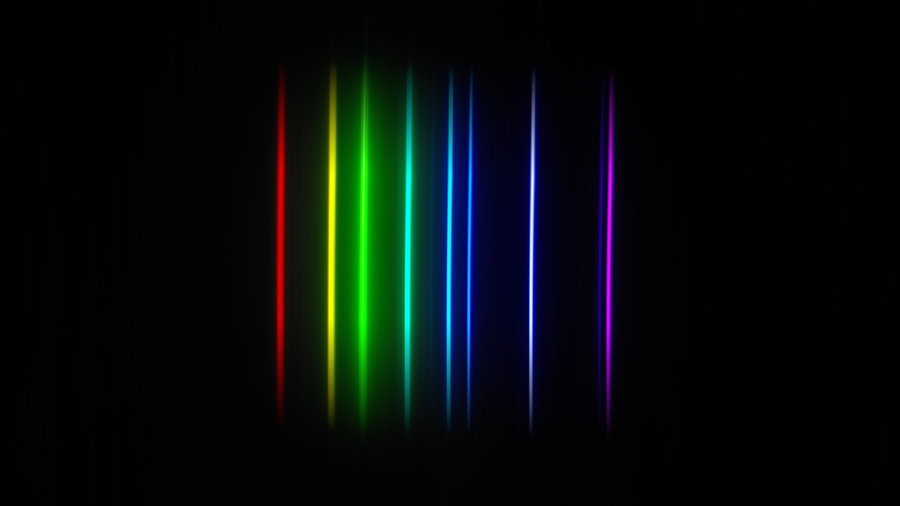
\includegraphics[scale=0.4]{images/spektrum.jpg}
  \caption{Emissionsspektrum einer Quecksilber-Cadmium-Dampflampe. \cite{2}}
  \label{fig:spektrum}
\end{figure}

\begin{figure}
  \centering
  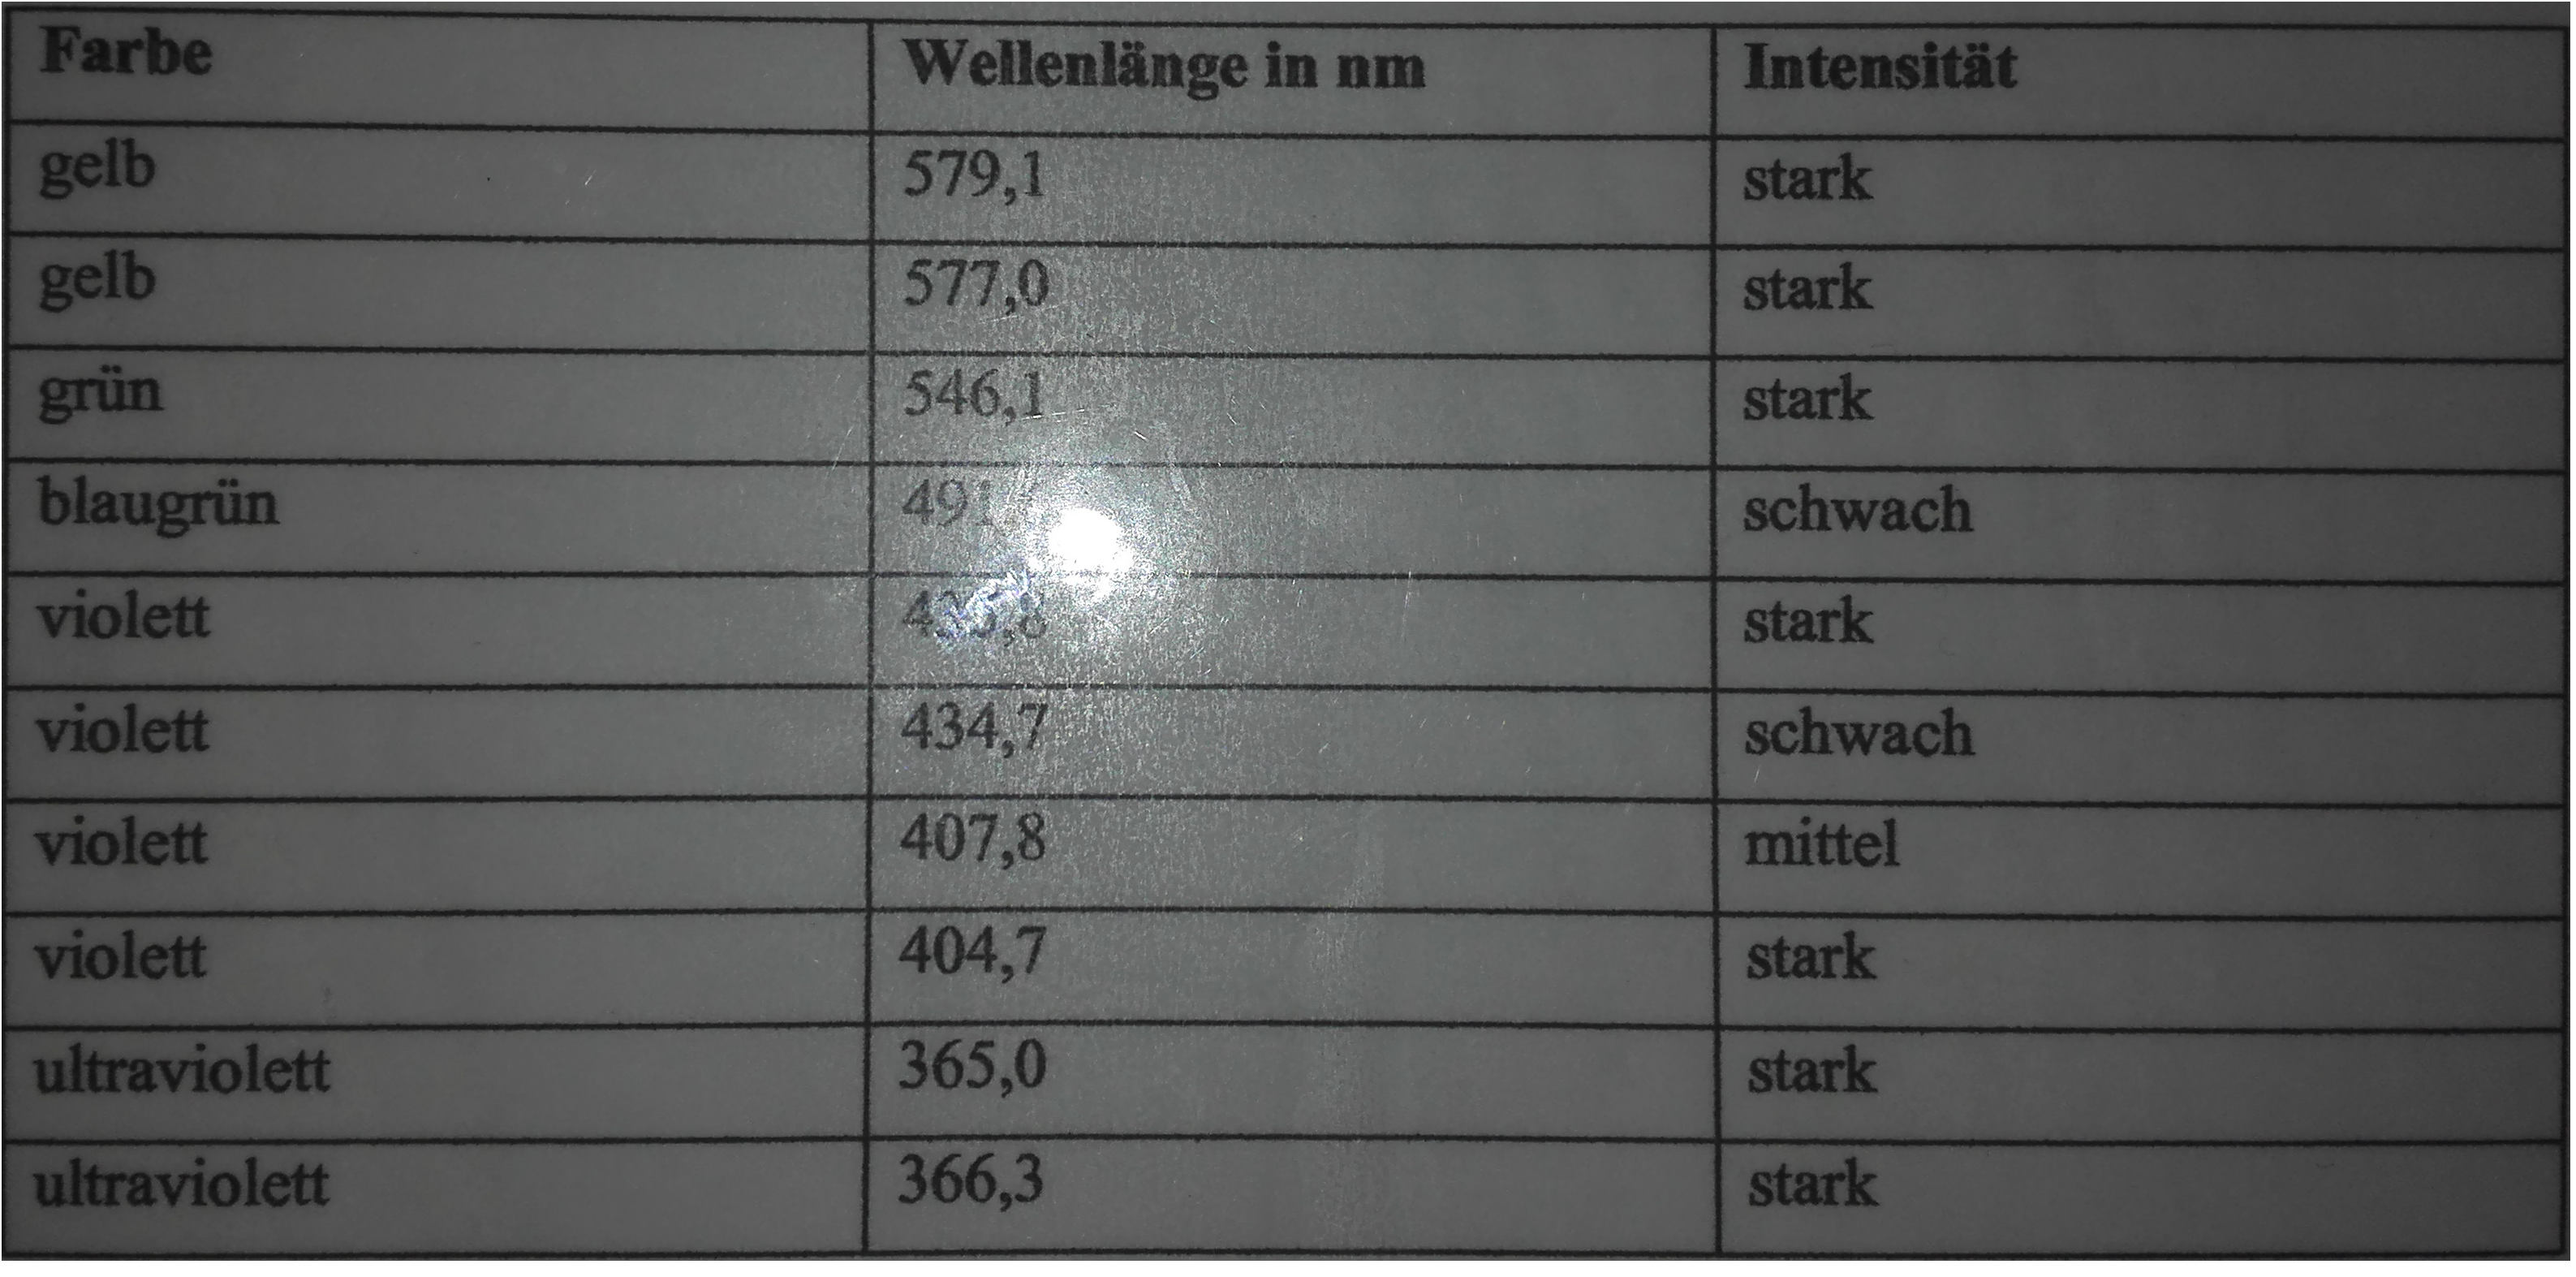
\includegraphics[scale=0.1]{images/Tabelle.png}
  \caption{Die Wellenlängen der Spektrallinien von Quecksilber: Fotografie der dem Versuch beiliegenden Tabelle}
  \label{fig:Etatabelle}
\end{figure}

\subsubsection{Berechnung der Brechungsindices $n_i$}

\begin{figure}
  \centering
  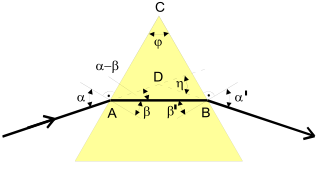
\includegraphics[scale=0.6]{images/Brechungsindex.png}
  \caption{Veranschaulichung der Winkelbeziehungen für die Berechnung der Brechungsindices $n_i$: Aus der Anleitung des Versuches \cite[23]{1}.}
  \label{fig:Brechungsindex}
\end{figure}

Die Brechungsindices $n_i$ in Abhängigkeit der Wellenlängen $\lambda_i$ werden nun nach dem snelliusschen Brechungsgesetz berechnet.
Die Winkelbeziehungen sind in Abbildung \ref{fig:Brechungsindex} dargestellt.
Für n ergibt sich dann folgende Formel:

\begin{equation}
  n = \frac{sin\frac{\eta + \upvarphi}{2}}{sin\frac{\upvarphi}{2}}
\end{equation}

Da es sich bei dem Winkel $\upvarphi$ um eine fehlerbehaftete Größe handelt, wird die Gauß'sche Fehlerfortpflanzung genutzt:
\begin{equation}
  \label{eqn:gauß}
  \Delta f = \sqrt{ \sum_{i=1}^N \left(\frac{\partial}{\partial x_i}\right)^2 \cdot \left(\Delta x_i\right)^2}
\end{equation}
Damit ergibt sich für den Fehler der Brechungsindices folgende Formel:
\begin{equation*}
  \increment n = \increment \upvarphi \cdot \Biggl(\frac{sin(\frac{\upvarphi}{2}) cos(\frac{\eta + \upvarphi}{2}) - cos(\frac{\upvarphi}{2}) sin (\frac{\eta + \upvarphi}{2})}{2 {sin(\frac{\upvarphi}{2})}^2} \Biggr)
\end{equation*}

Diese werden mit uncertainties berechnet.
Die Ergebnisse sind in Tabelle \ref{tab:Brechungsindex} zusammengefasst.

\begin{table}
  \caption{Die Brechungsindices $n_i$ in Abhängigkeit von den Wellenlängen $\lambda_i$}
  \label{tab:Brechungsindex}
  \centering
  \sisetup{table-format=3.1}
  \begin{tabular}{S [table-format=3.1]
    S [table-format=1.2]
    @{${}\pm{}$}
    S [table-format=1.2]
    }
    \toprule
    {$\lambda_i \:/\: \si{\nano\metre}$} & \multicolumn{2}{c}{$n_i$} \\
    \midrule
    643.85 & 1.75 & 0.00 \\
    576.96 & 1.76 & 0.00 \\
    546.07 & 1.77 & 0.00 \\
    508.58 & 1.78 & 0.00 \\
    479.99 & 1.78 & 0.00 \\
    467.82 & 1.79 & 0.00 \\
    435.83 & 1.80 & 0.00 \\
    404.65 & 1.81 & 0.00 \\
    \bottomrule
  \end{tabular}
\end{table}

Der Brechungsindex nimmt mit zunehmender Wellenlänge ab.
Es handelt sich also um eine normale Dispersion.

\subsection{Bestimmung der Dispersionskurve}

Nun muss den bestimmten Brechungsindices eine entsprechende Dispersionskurve zugewiesen werden.
Die Quadrate der Brechungsindices wurden dafür in Abbildung \ref{fig:Brechungsplot} gegen die Wellenlänge aufgetragen.


\begin{figure}
  \centering
  \includegraphics[scale=0.6]{build/plot3.pdf}
  \caption{Die Quadrate der Brechungsindices in Abhängigkeit der Wellenlänge.}
  \label{fig:Brechungsplot}
\end{figure}

Nun werden für die Gleichungen \ref{eqn:4} und \ref{eqn:5} die entsprechenden $A_i$, bzw $A'_i$ -Werte gefittet.
Dies erfolgt mit numpy und es ergeben sich folgende Werte:

\begin{align*}
  A_0 &= 2.99 \pm 0.01 \\
  A_2 &= 42087.30 \pm 2904.23 \si{\square\metre}\\
  A'_0 &= 3.36 \pm 0.02 \\
  A'_2 &= (7.59 \pm 0.84) \times 10^{-7} \si{\per\square\metre}\\
\end{align*}

Die gefitteten Kurven sind in den Abbildungen \ref{fig:fit1} und \ref{fig:fit2} zu sehen.

\begin{figure}
  \centering
  \includegraphics[scale=0.6]{build/plot1.pdf}
  \caption{Mit Gleichung \ref{eqn:4} gefittete Dispersionskurve.}
  \label{fig:fit1}
\end{figure}
\begin{figure}
  \centering
  \includegraphics[scale=0.6]{build/plot2.pdf}
  \caption{Mit Gleichung \ref{eqn:5} gefittete Dispersionskurve.}
  \label{fig:fit2}
\end{figure}

Mit diesen wird jetzt die Summe der Abstandsquadrate nach folgenden Formel berechnet:

\begin{align*}
  s^2_n &= \frac{1}{z - 2} \sum_{i=1}^z \left\{n^2(\lambda_i) - A_0 - \frac{A_2}{\lambda_i^2} \right\}^2
  \shortintertext{bzw.} \\
  s^2_{n'} &= \frac{1}{z - 2} \sum_{i=1}^z \left\{n^2(\lambda_i) - A'_0 - A'_2\lambda_i^2 \right\}^2
\end{align*}

Mit z = Anzahl der Messwerte.
Mit entsprechend eingesetzten Werten ergibt sich:

\begin{align*}
  s^2_n &= 1.57 \times 10^{-4} \\
  s^2_{n'} &= 0.22
\end{align*}

Da die Summe der Abweichungsquadrate für die Dipersionskurve, welche durch Gleichung \ref{eqn:4} beschrieben wird, deutlich kleiner ist,
beschreibt diese das Dispersionsverhalten des Prismas genauer.
Somit ergibt sich für die in Abbildung \ref{fig:plot4} zu sehende Dispersionskurve
\begin{equation}
  n(\lambda) = \sqrt{2.99 + \frac{42087 \si{\square\metre}}{{\lambda}^2}} .
  \label{eqn:disp}
\end{equation}

\begin{figure}
  \centering
  \includegraphics[scale=0.8]{build/plot4.pdf}
  \caption{Mit Gleichung \ref{eqn:disp} berechnete Dispersionskurve.}
  \label{fig:plot4}
\end{figure}

\subsection{Abbesche Zahl}

Die Abbesche Zahl stellt ein Maß der Farbzerstreuung für ein gegebenes Material dar.
In diesem Fall für Schwerflint SF14.
Durch die zuvor berechnete Dispersionsgleichung kann nun mit der folgenden Formel:

\begin{equation}
  \nu = \frac{n_d - 1}{n_F - n_C}
\end{equation}

die Abbesche Zahl $\nu$ berechnet werden.
Dabei stellen die Konstanten $n_D$, $n_F$ und $n_C$ die entsprechenden Brechungsindices zu den sogenannten Fraunhoferschen Linien mit folgenden Werten dar:

\begin{align*}
  \lambda_C &= \SI{656}{\nano\metre} & n_C &= 1.76\\
  \lambda_d &= \SI{589}{\nano\metre} & n_D &= 1.76\\
  \lambda_F &= \SI{486}{\nano\metre} & n_F &= 1.78
\end{align*}

Für die Abbesche Zahl ergibt sich dann:

\begin{align*}
  \nu = 33.52
\end{align*}

\subsection{Auflösungsvermögen}

Das Auflösungsvermögen eines Prismen-Spektralapparates ist die Fähigkeit dessen zwei benachbarte Wellenlängen mit dem Wellenlängenunterschied $\Delta\lambda$ gerade noch auflösen, bzw. trennen zu können.
Das Auflösungsvermögen A wird damit folgendermaßen definiert:

\begin{align}
  A &:= \frac{\lambda}{\Delta\lambda}
  \intertext{Es kann gezeigt werden, dass das Auflösungsvermögen durch folgende Gleichung gegeben ist:}
  A &=  b \frac{d}{d\lambda} n(\lambda)
  \label{eqn:auflosung}
\end{align}

Hierbei ist b die Basislänge des Prismas.
Diese wurde nicht explizit gemessen und wird der Anleitung \cite[28]{1} mit $b = \SI{3}{\centi\metre}$ entnommen.
Die Ableitung von $n(\lambda)$ nach $\lambda$  ergibt:

\begin{equation}
  \frac{d}{d\lambda} n(\lambda) = \frac{d}{d\lambda} \sqrt{A_0 + \frac{A_2}{\lambda^2}} = - \frac{A_2}{\lambda^3 \sqrt{A_0 + \frac{A_2}{\lambda^2}}}
\end{equation}

Setzt man dies in die Gleichung \ref{eqn:auflosung} so ergeben sich folgende Werte, die in Tabelle \ref{tab:Auflösungsvermögen} dargestellt sind.

\begin{table}
  \centering
  \caption{Die berechneten Auflösungsvermögen für die Fraunhoferschen Linien}
  \label{tab:Auflösungsvermögen}
  \sisetup{table-format=4.2}
  \begin{tabular}{c c c}
    \toprule
    {$\text{Linie}$} & {$\lambda \:/\: \si{\nano\metre}$} & {$\text{Auflösungsvermögen}$} \\
    \midrule
    $\lambda_C$ & 656 &  2547.33 \\
    $\lambda_D$ & 589 &  3505.91 \\
    $\lambda_F$ & 486 &  6184.41 \\
    \bottomrule
  \end{tabular}
\end{table}

\subsection{Nächstgelegene Absorptionsstelle}
Zur Bestimmung der nächstgelegenen Absorptionsstelle ${\lambda}_1$ wird zunächst \ref{eqn:3} mit \ref{eqn:4} verglichen.
So ergibt sich für die Koeffizienten :
\begin{align*}
  A_0 &= 1+ \frac{N_1 {q_1}^2 {{\lambda}_1}^2}{4 {\pi}^2 c^2 {\epsilon}_0 m_1}
  \intertext{und}
  A_2 &= \frac{N_1 {q_1}^2 {{\lambda}_1}^4}{4 {\pi}^2 c^2 {\epsilon}_0 m_1}
\end{align*}
Nun werden diese Koeffizienten verglichen und nach ${\lambda}_1$ aufgelöst, wodurch sich folgende Formel für die nächstgelegene Absorptionsstelle ergibt:
\begin{equation}
  {\lambda}_1 = \sqrt{\frac{A_2}{A_0 - 1}}.
  \label{eqn:lambda1}
\end{equation}
Nun werden die Werte in \eqref{eqn:lambda1} eingesetzt.
Für den Fehler wird mit \eqref{eqn:gauß} folgende Formel hergeleitet:
\begin{equation*}
  \increment {\lambda}_1 = \sqrt{\frac{{(\increment A_2)}^2}{4 A_2 (A_0 - 1)} + \frac{A_2 {(\increment A_0)}^2}{4 {(A_0 -1 )}^{3}}}
\end{equation*}
So ergibt sich für die Absorptionsstelle:
\begin{equation*}
    {\lambda}_1 = 145 \pm 5 \: \si{\nano\metre}
\end{equation*}
berechnet. Dies entspricht einer Wellenlänge im ultravioletten Bereich.
